\documentclass[10pt,aspectratio=169,mathserif]{beamer}	

\usepackage{amsmath, amsfonts, amssymb, bm}
\usepackage{ctex}
\usepackage{color}
\usepackage{graphicx, hyperref, url}
\usepackage{ecnu}
\usepackage{booktabs}

\beamertemplateballitem	

\title{NVIDIA新架构GPU为机器学习应用带来的性能提升的研究与评估}
\subtitle{毕业设计答辩}

\author[Altair Liu]{
	刘子汉 \\
	{\small {10152130243@stu.ecnu.edu.cn}}
}

\institute[ECNU]{
	华东师范大学 \\
	计算机科学与软件工程学院\\
	计算机科学与技术系
}

\date[2019.05.15]{
	2019.05.15
}

\begin{document}
	\begin{frame}
	\titlepage
	\end{frame}

	\section{大纲}
	\begin{frame}
		\frametitle{大纲}
		\tableofcontents
	\end{frame}

	\section{简介}
	\begin{frame}
		\frametitle{简介}
		\begin{itemize}
			\item 2017Q3,NVIDIA发布新架构GPU Tesla V100及其中的张量核心,且宣称矩阵乘加性能提升达9.3倍。
			\item Stefano等人的研究中,相同情况下其新架构GPU性能提升幅度仅有4-6倍,如下图所示。
			\begin{figure}
				\centering
				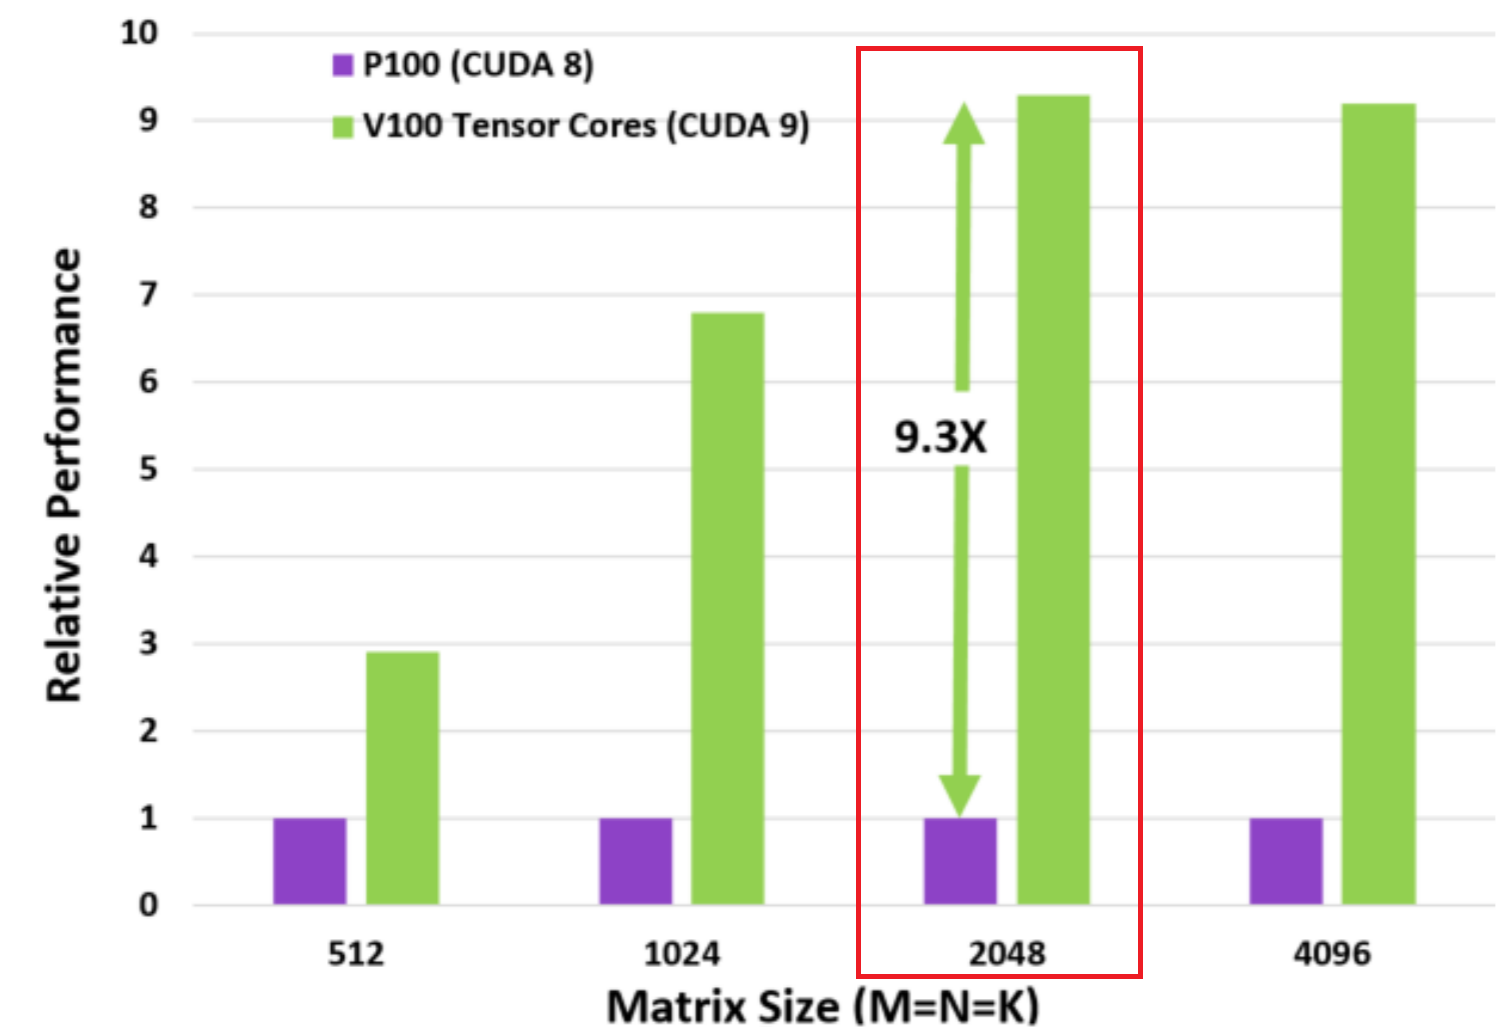
\includegraphics[width=6cm]{figures/VoltaGemmPerf.jpg}
				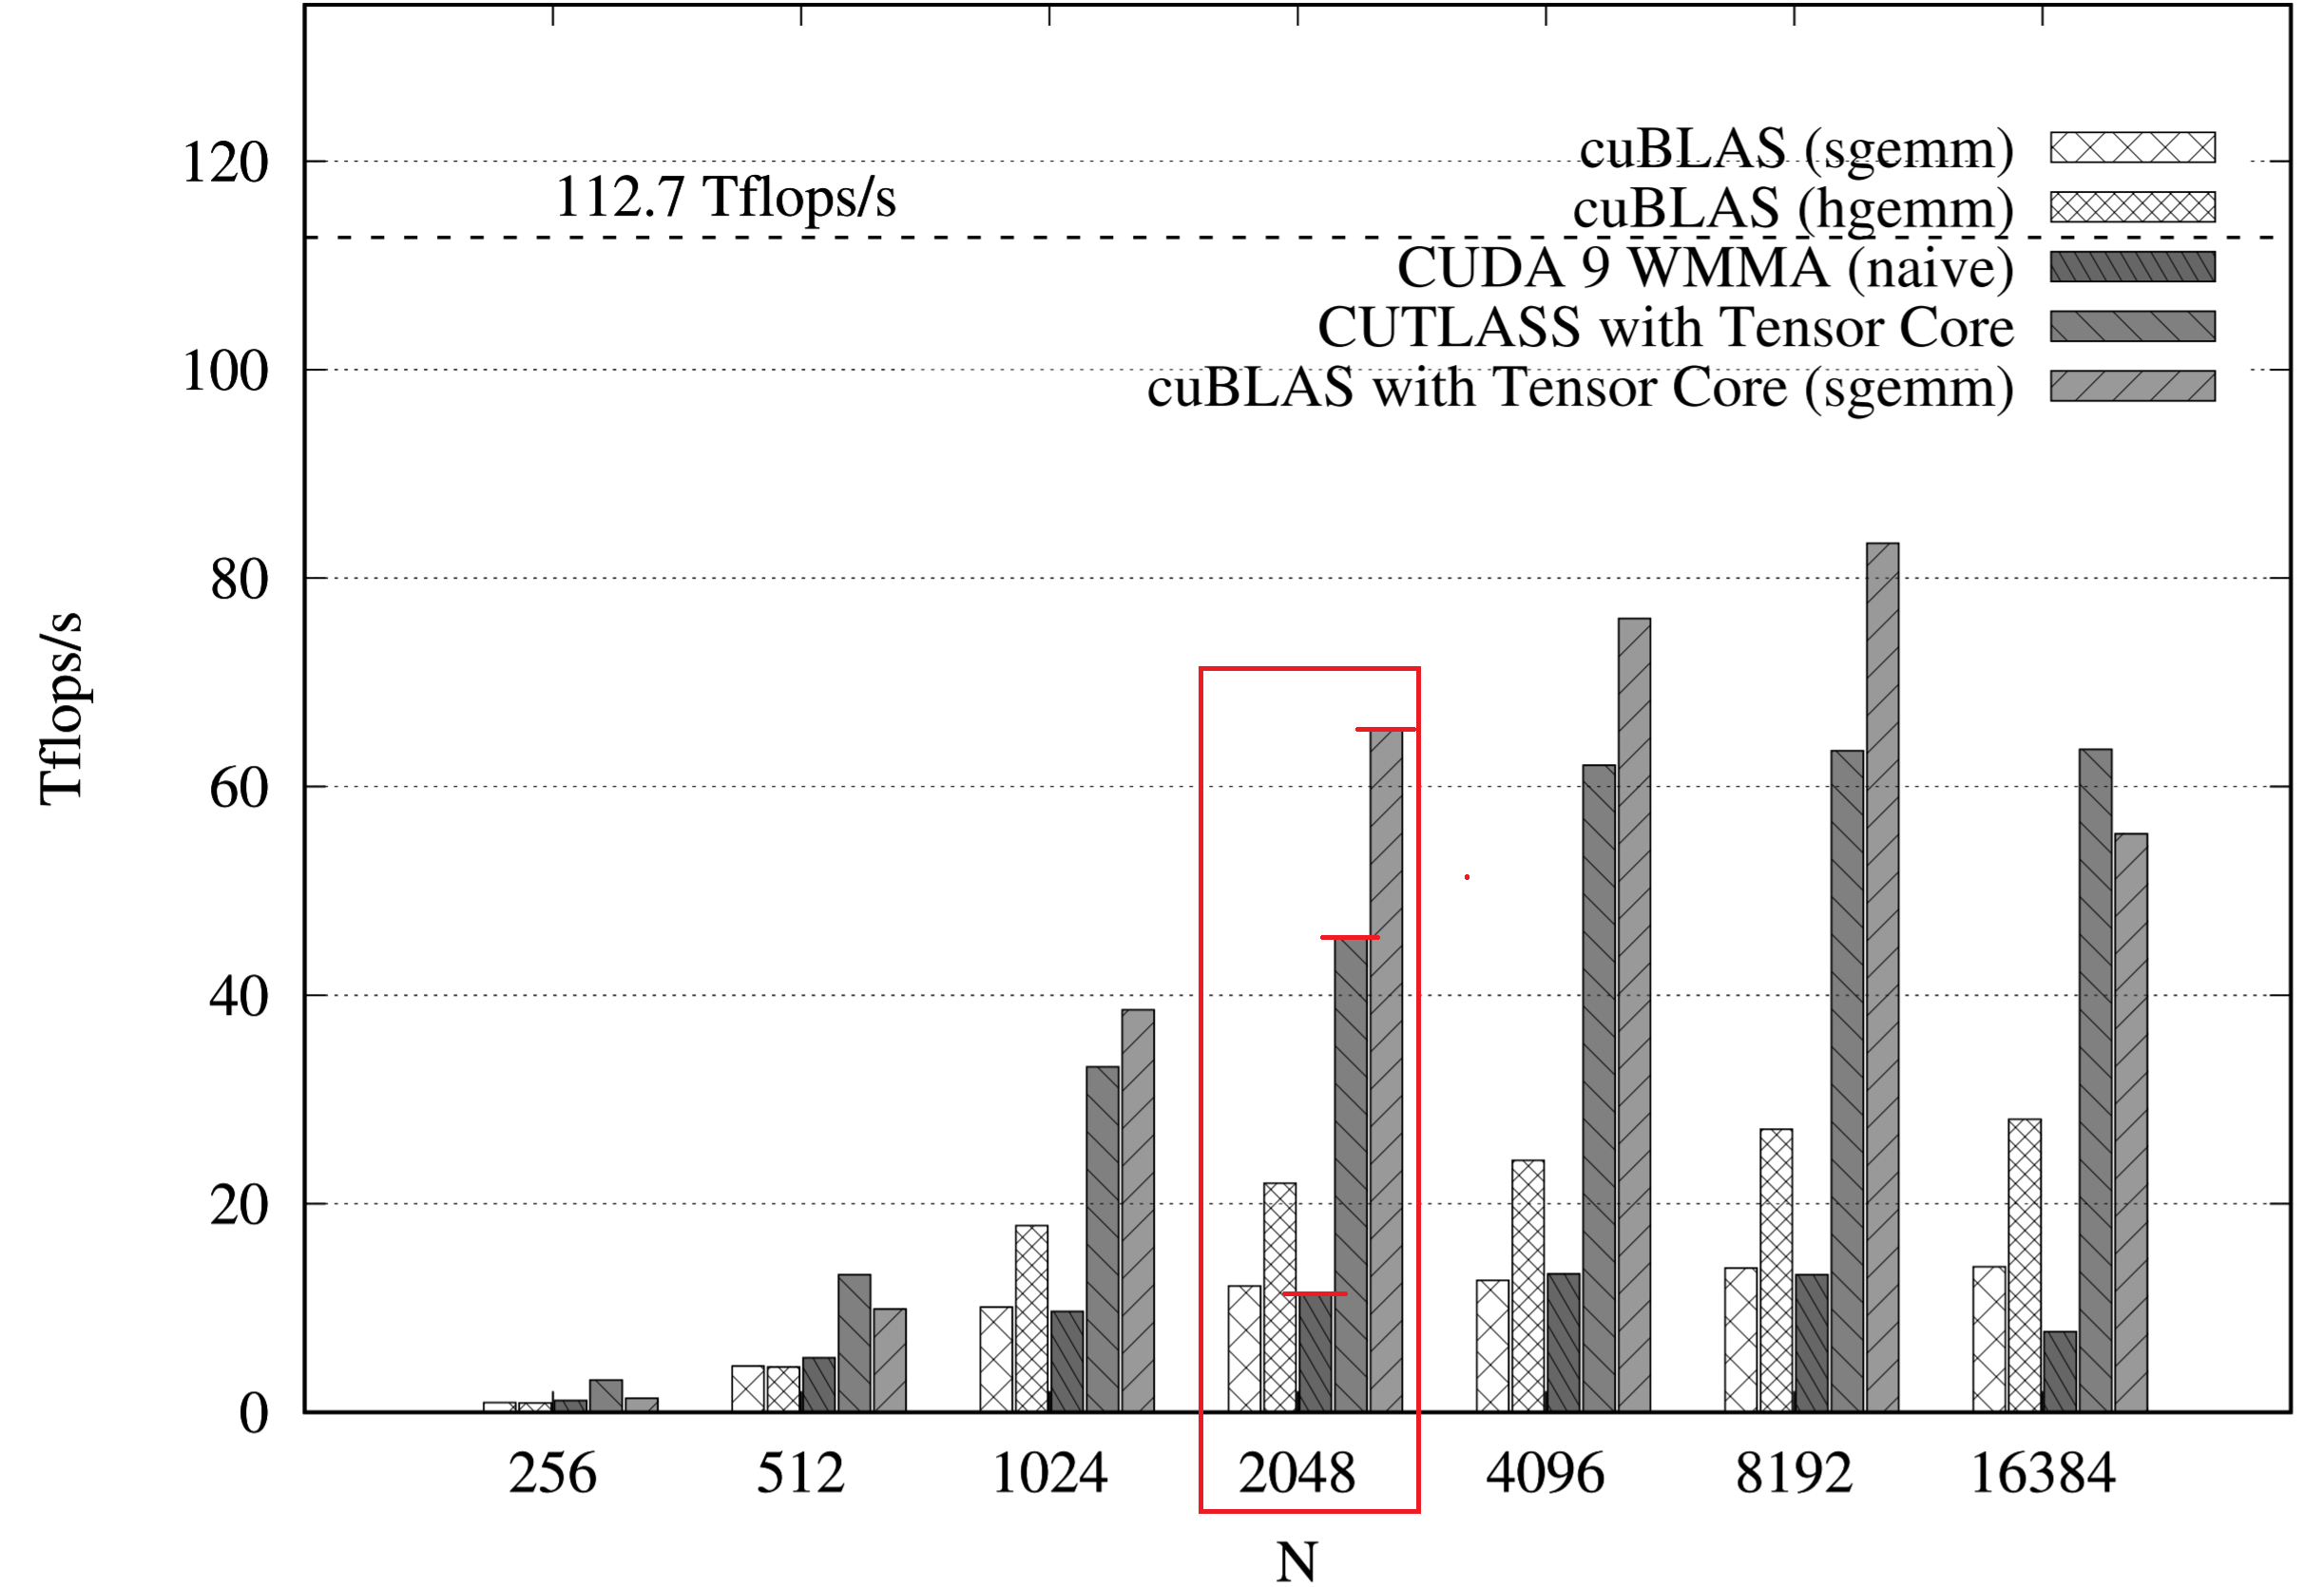
\includegraphics[width=6cm]{figures/ActualGemmPerf.jpg}
				\caption{官方白皮书性能与实际研究中性能比较}\label{Fig.COMPARE}
			\end{figure}
		\end{itemize}
	\end{frame}
	\begin{frame}
		\frametitle{简介}
		\begin{itemize}
			\item 在实际使用框架如Tensor Flow搭建的模型中提升幅度更低。在特定结构的网络中开启张量核心仅能带来60\%-80\%的提升。
			\item {\bf 本文将从Python源码、CUDA C源码、PTX中间代码、SASS硬件代码的层面,借助卷积神经网络和支持向量机这两种经典的应用,对新架构GPU为机器学习应用带来的性能提升进行评估,尝试在代码层面进行优化,并提出设想。}
			\item 具体评估的应用遵循自底向上的结构:
				\begin{itemize}
					\item Benchmark样例(矩阵乘法、\textbf{矩阵乘加}、卷积运算)
					\item 基于CUDA源码的应用(卷积神经网络、支持向量机)
					\item 基于Tensor Flow的应用(卷积神经网络)
				\end{itemize}
			\item 除训练过程外,最后使用TensorRT以及Jetson对部署、推理过程进行优化。
		\end{itemize}
	\end{frame}

	\section{背景}
	\begin{frame}
		\frametitle{背景}
		\begin{itemize}
			\item 机器学习与GPU:目前绝大部分机器学习应用都需要GPU进行加速,而NVIDIA GPU长期占据高性能计算的市场。
			\item NVIDIA GPU结构:自上而下分为图形处理器簇(GPC)、纹理处理器簇(TPC)、流多处理器(SM)。流多处理器中有若干种处理单元如整数、浮点、逻辑单元。
			\item 伏特架构/图灵架构:在流处理器中加入了张量核心的新架构,分别对应计算能力7.0与7.5,图灵是消费级芯片,屏蔽了一些硬件。
			\item 张量核心:专为矩阵乘加设计的硬件,以半精度浮点进行运算(FP16),以wmma指令批量执行原先整数点积指令与累加指令执行的任务。
			\item 纹理内存:访问时将二维空间上的周围数据加载进入缓存,其余存储系统为加载一行。
			\item 线程束:内含32个GPU线程,作为基本的调度、同步单元。
			\item TensorRT与Jetson:TensorRT是一个GPU推理引擎,用于优化训练完毕的模型,加速推理。Jetson是NVIDIA开发的面向嵌入式应用的芯片。
		\end{itemize}
	\end{frame}

	\section{相关工作}
	\begin{frame}
		\begin{itemize}
			\item GPGPU-SIM:PTX中间代码执行的软件层面模拟。
			\item SMart, PerfSIM:SASS硬件代码执行的软件层面模拟以及RTL仿真。
			\item ThunderSVM:并行支持向量机。
			\item Leng J.:大型集群的性能、能耗优化。
			\item Mahmoud K.:访存优化
			\item ?张量核心
		\end{itemize}
	\end{frame}

	\section{实验平台}
	\begin{frame}
		\frametitle{实验平台}
		\begin{table}
			\centering
			\caption{实验平台}
			\begin{tabular}{cc}
				\toprule
				项目	&	内容\\
				\midrule
				CPU		&	AMD Ryzen ThreadRipper 2990WX 32C64T @ 3.0GHz\\
				主板		&	MSI X399\\
				内存		&	CORSAIR DDR4 3200 @ 16-15-15-15-34-1T 128GB\\
				GPU		&	NVIDIA Geforce RTX 2080TI (Turing)\\
				硬盘		&	INTEL750 NVMe PCIe 1.2TB * 2 @ RAID 0\\
				系统		&	Windows 10 64-bit build 17763\\	
				CUDA	&	Ver. 10.1, 10.0, 9.2, 9.0\\
				CUTLASS & Ver. 1.2, 1.3\\
				其他		&	Jetson TX2 $ * $\\
				\bottomrule
			\end{tabular}
		\end{table}
	\end{frame}
	
	\section{实验内容}
	\subsection{Benchmark}
	\subsubsection{矩阵乘加}
	\begin{frame}
		\frametitle{Benchmark::矩阵乘加}
		由于新老架构GPU在参数、外围设备等方面均有改进,为了重点研究张量核心的性能,本文中的实验均在RTX 2080TI上通过开启/关闭张量核心进行评估。
		\begin{figure}
			\centering
			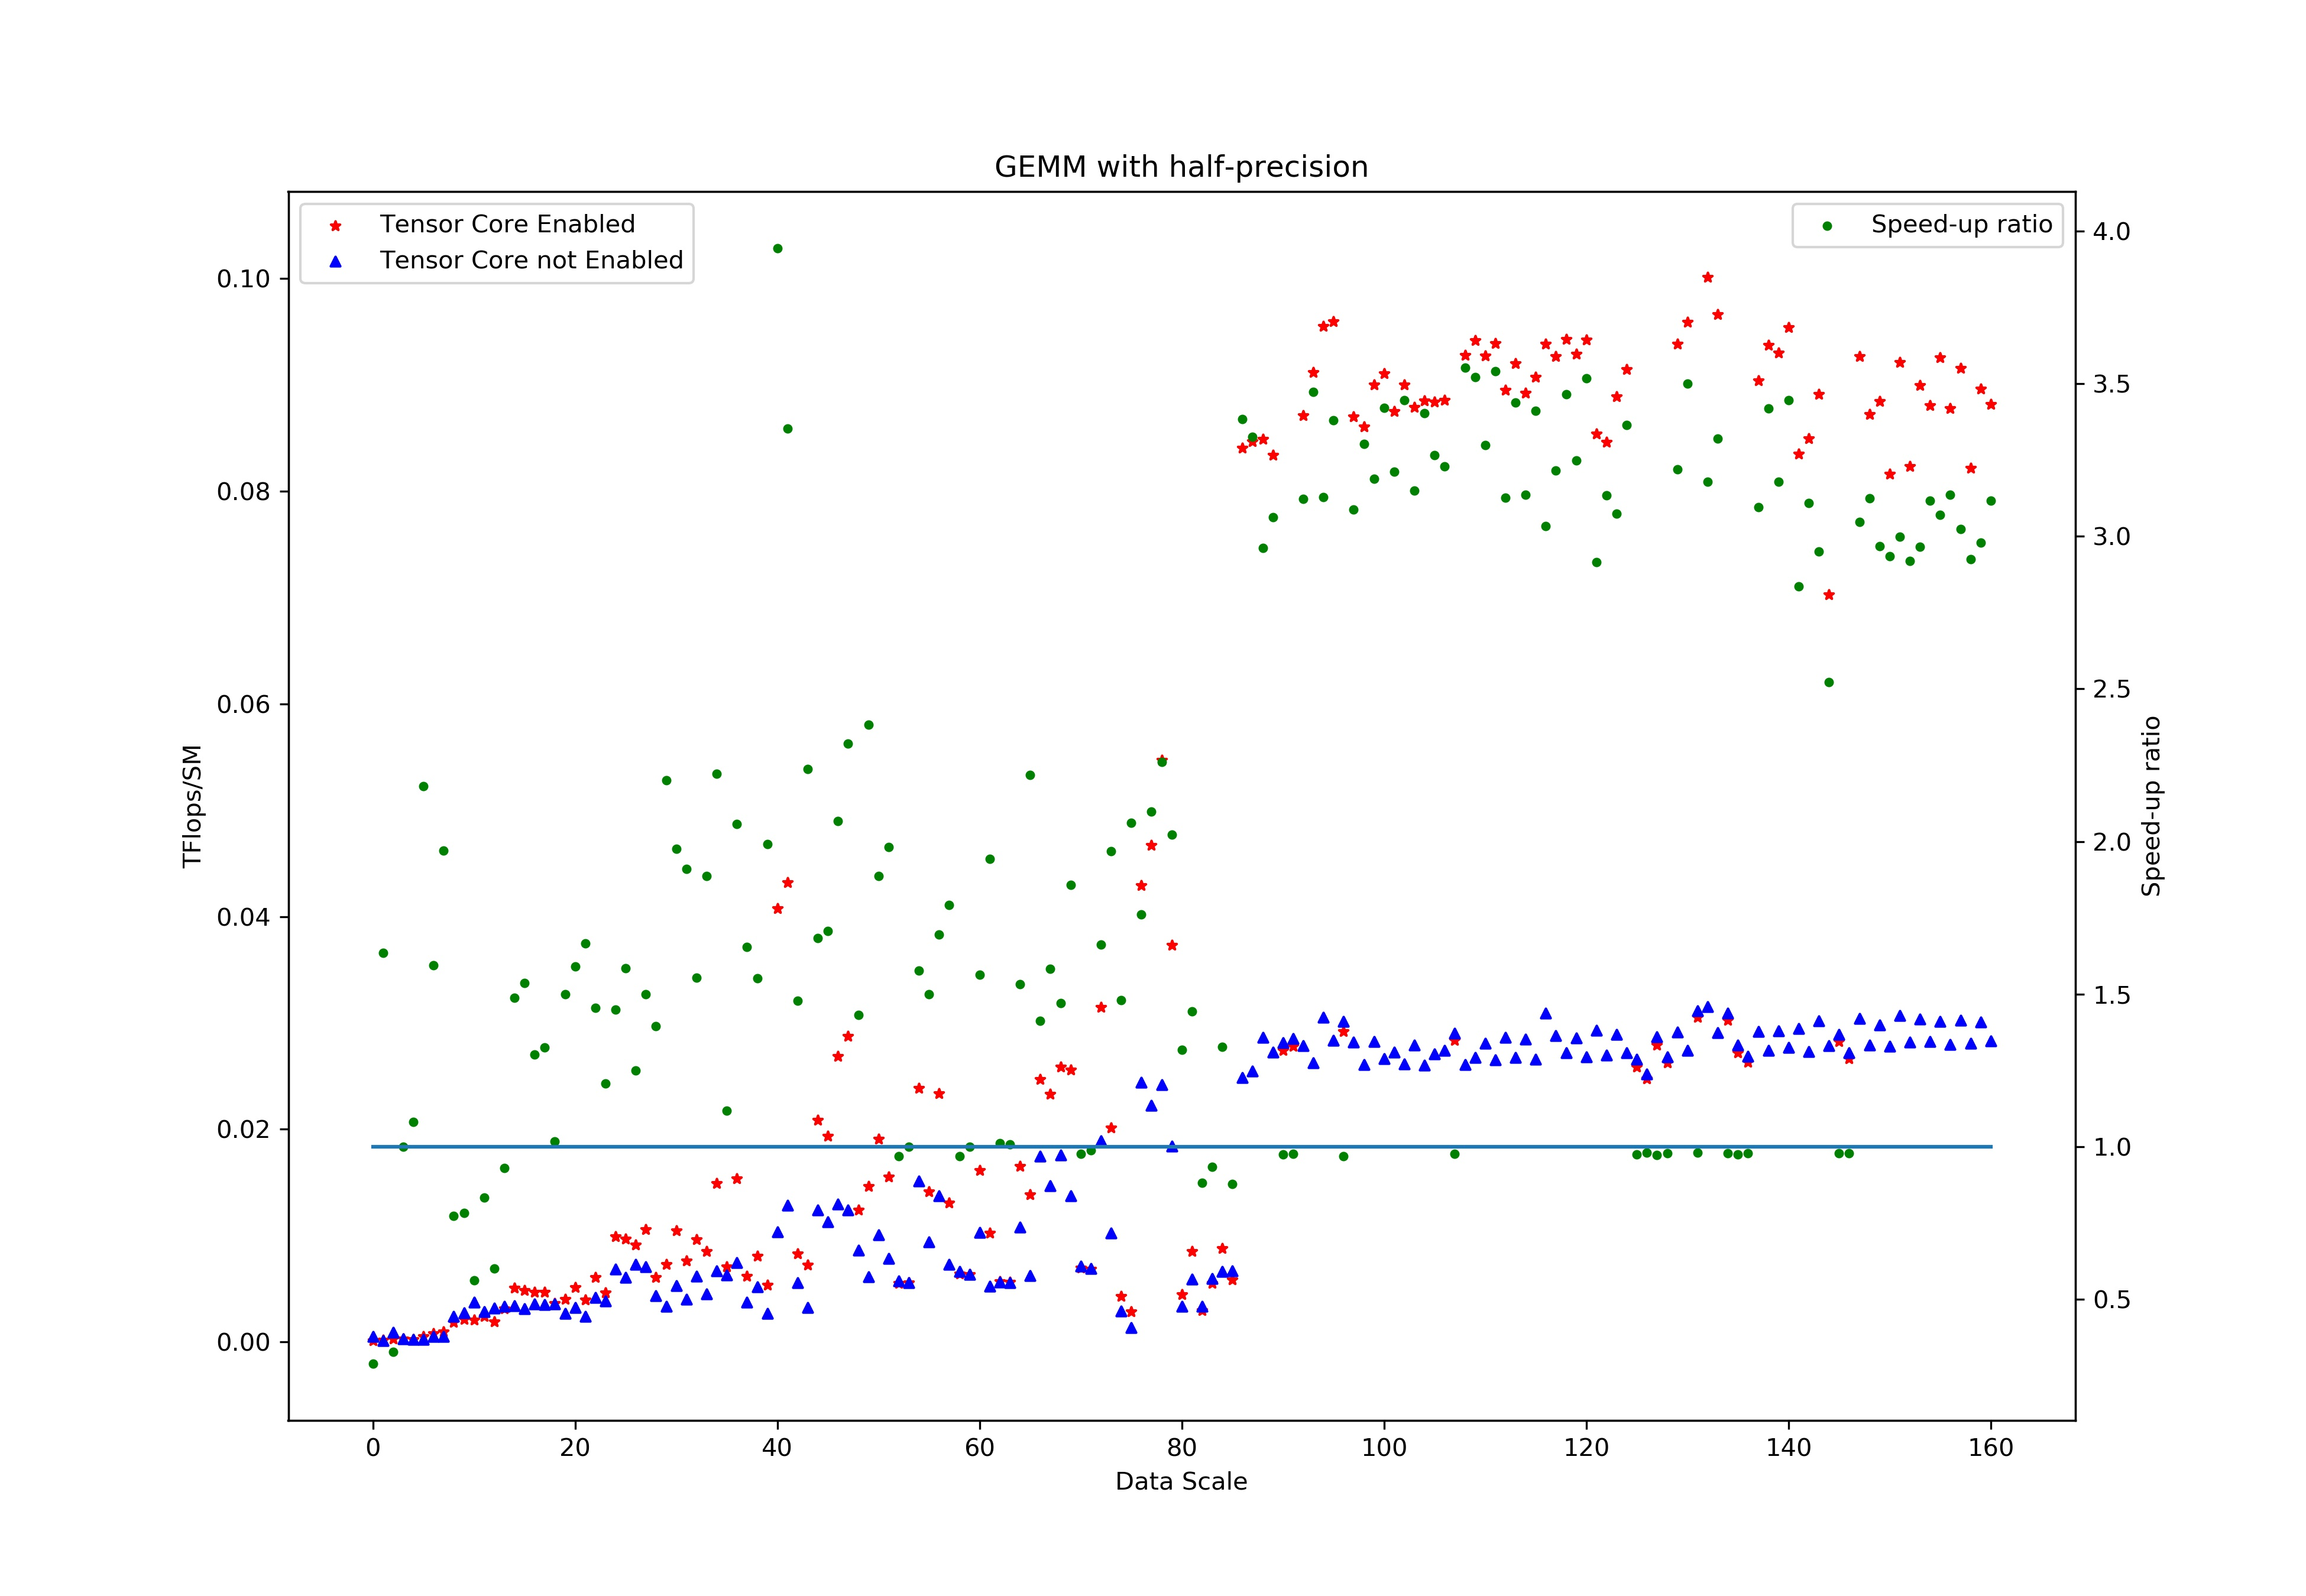
\includegraphics[width=5.5cm]{figures/GEMM-Half-TF.jpg}
			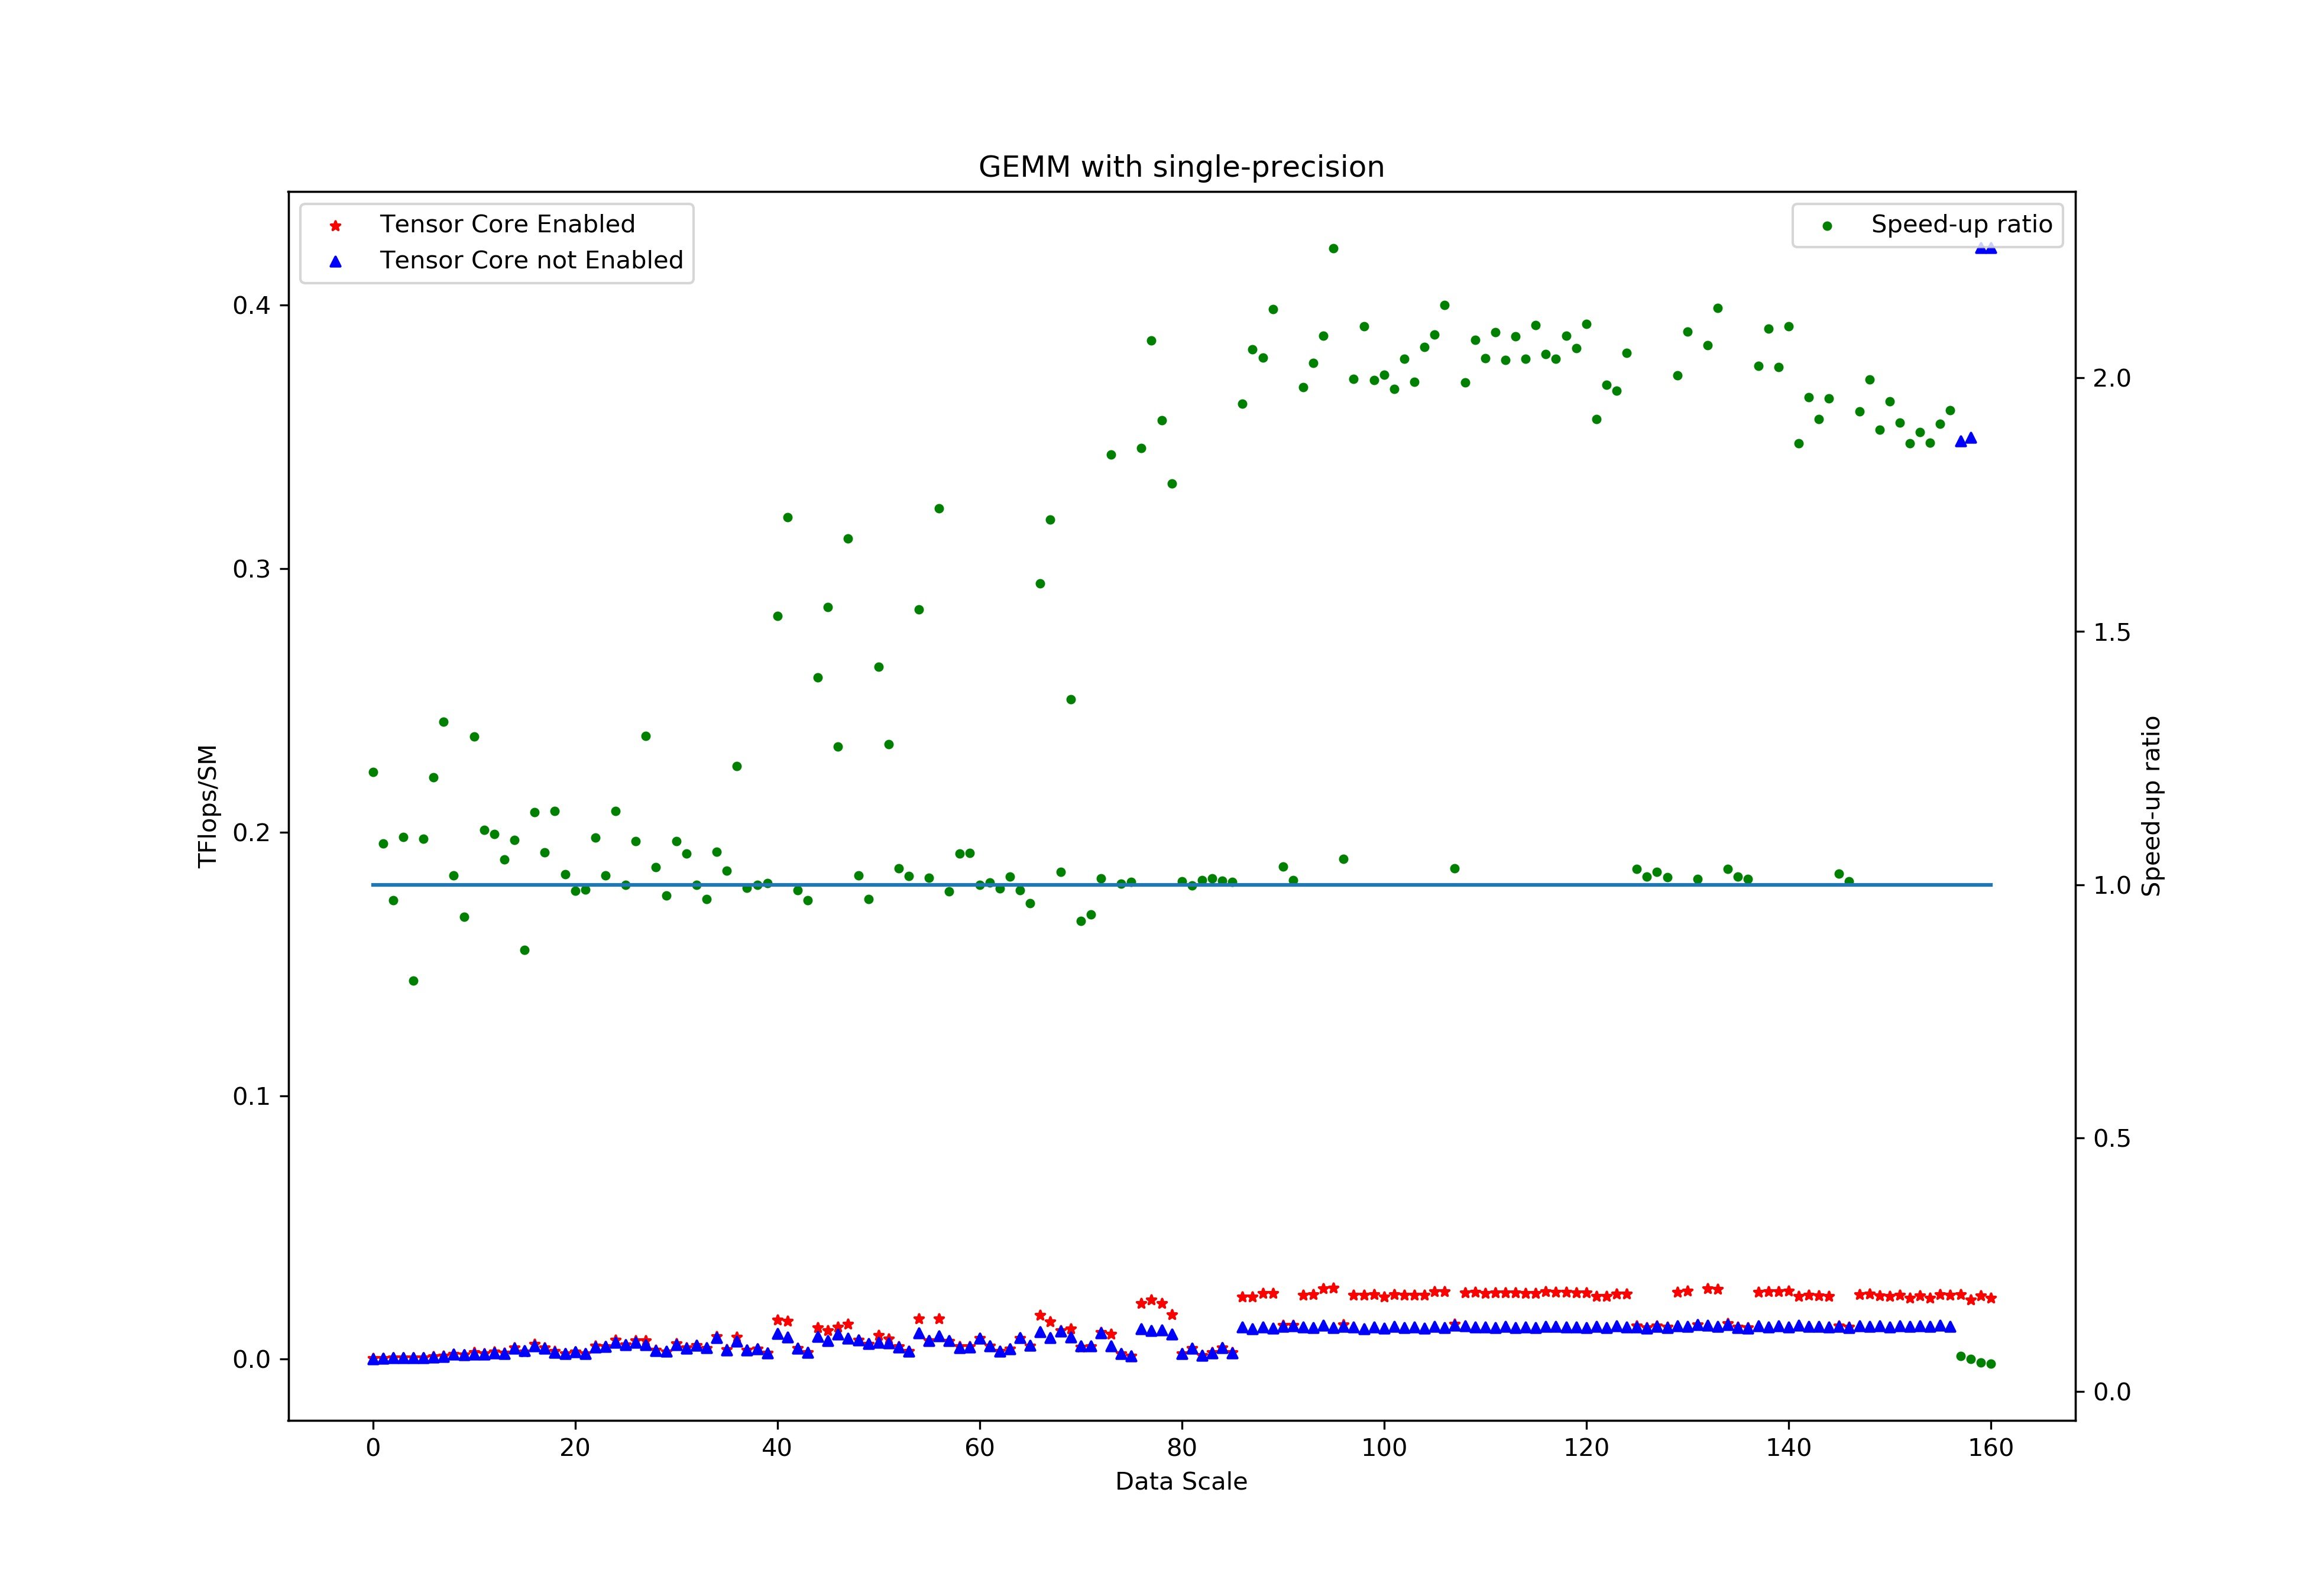
\includegraphics[width=5.5cm]{figures/GEMM-Single-TF.jpg}
			\caption{不同计算量下开启和关闭张量核心的性能(半精度/单精度)}\label{Fig.GEMM}
		\end{figure}
		在计算量较大的情况下,开启张量核心后半精度性能提升3-4倍,单精度性能提升2倍。
	\end{frame}
	
	\begin{frame}
		\frametitle{Benchmark::矩阵乘加}
		使用nvprof和NSight进行分析:
		\begin{table}
			\centering
			\caption{开启/关闭张量核心的对比}
			\begin{tabular}{ccc}
				\toprule
				项目	&	开启张量核心 & 关闭张量核心\\
				
				\midrule
				CUDA设备同步耗时 & \textbf{186.15s} & 543.51\\
				CUDA设备同步耗时占比 & \textbf{79.29\%} & 91.40\%\\
				一次乘加所需计算指令 & \textbf{一条wmma} & 若干条idp/idp4a+累加指令\\
				每条计算指令延迟 & \textbf{wmma: 8时钟周期} & idp/idp4a: 4时钟周期\\
				上下文切换时间占比 & \textbf{44.39\%} & 52.52\%\\
				\bottomrule
			\end{tabular}
		\end{table}
		开启张量核心后设备同步、上下文切换等死时间减少,原因为张量核心整合多次计算为一次。
	\end{frame}

	\begin{frame}
		\frametitle{Benchmark::矩阵乘加}
		根据官方文档说明,张量核心对于矩阵裁切形状较为敏感,故将实验结果按加速比排序并按形状特征着色,形状特征分为:能够被32整除、能够被8整除,无法被整除。
	\end{frame}

	\subsubsection{矩阵乘法}
	\begin{frame}
		\frametitle{Benchmark::矩阵乘法}
	\end{frame}
	\subsubsection{卷积}
	\begin{frame}
		\frametitle{Benchmark::卷积}
	\end{frame}
	\subsection{CUDA}
	\subsubsection{卷积神经网络(cuDNN)}
	\begin{frame}
		\frametitle{CUDA C::卷积神经网络}
	\end{frame}
	\subsubsection{支持向量机(SMO-SVM)}
	\begin{frame}
		\frametitle{CUDA C::支持向量机}
	\end{frame}
	
	\subsection{TensorRT}
	\begin{frame}
		\frametitle{TensorRT与Jetson优化推理}
	\end{frame}
	
	\subsection{Tensor Flow}
	\begin{frame}
		\frametitle{Tensor Flow-GPU::LeNet-5卷积神经网络}
	\end{frame}
	
	\section{总结}
	\begin{frame}
		\frametitle{总结}
	\end{frame}

	\section{参考文献}
	\begin{frame}
		\frametitle{参考文献}
		\begin{thebibliography}{99}
			\bibitem{VOLTAWHITEPAPER} NVIDIA. (2017).\\
			{\bf NVIDIA TESLA V100 GPU ARCHITECTURE} \\
			NVIDIA Corp., pages 14-15, August, 2017.
		\end{thebibliography}
	\end{frame}

	
\end{document}


